%%% Local Variables: 
%%% mode: latex
%%% TeX-master: t
%%% End: 

\chapter{其他工作}
\section{HGCal模块组装}

HGCal全称高颗粒度量能器(High Granularity Calorimeter),是CMS实验中为了迎接高亮度大型强子对撞机(HL-LHC)所进行的二期阶段升级项目,这个项目主要针对的是对CMS探测器端盖部分的量能器进行升级。

HL-LHC的设计目标是在第三阶段停机结束后,经过十年的运行取数,最终获得总积分亮度为3000~\si{fb^{-1}}的数据。为了达到这个目标,LHC的瞬时亮度可以达到~\num{5e34}~\si{\cm^{-2}\s^{-1}},是现在的三倍,在如此高的瞬时亮度条件下,每次质子数团碰撞可以产生140--200个堆积事例。与此同时,对撞产生的粒子以及这些粒子和探测器中的物质相互作用产生的辐射会对探测器中的电子学设备产生极大地损坏。在端盖位置,辐射本底预计可以达到~\num{1.5e16}~\si{n/cm^{2}},是目前的100倍。

\begin{figure}[!htbp]
    \centering
    %trim option's parameter order: left bottom right top
    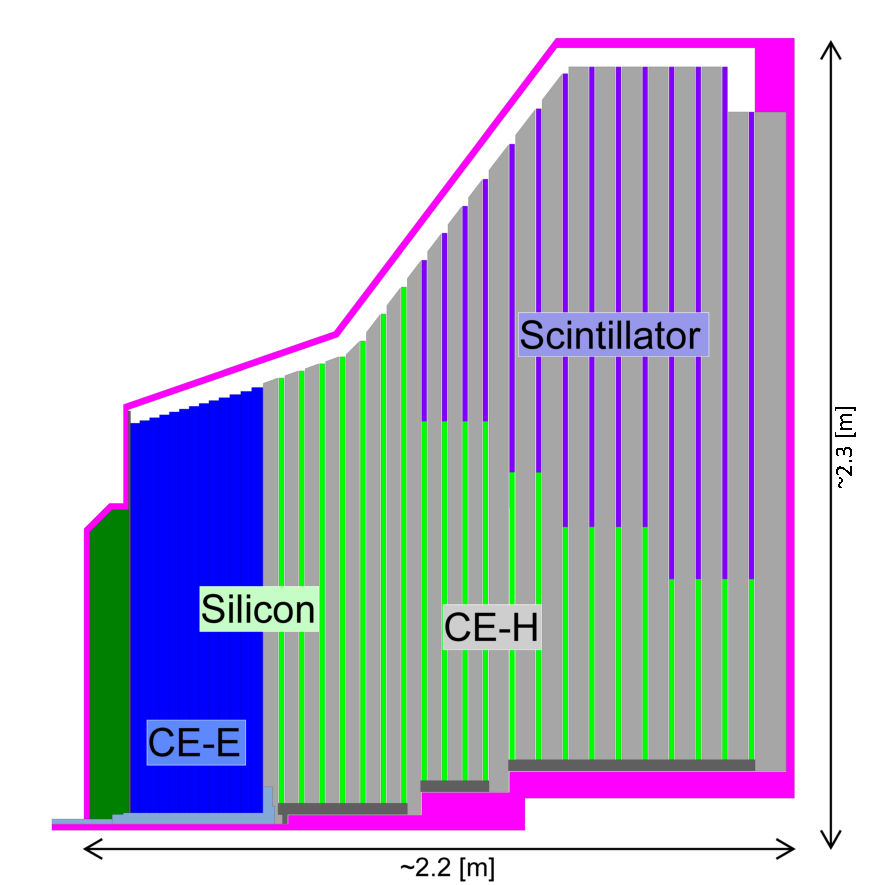
\includegraphics[width=0.7\textwidth]{figures/chapter05/HGCal.pdf}
    \bicaption{\quad \centering 用于 HL-LHC 升级的 CMS HGCal 探测器~\cite{Martelli:2281440}}{\quad \centering The CMS HGCal detector for HL-LHC upgrade~\cite{Martelli:2281440}}
    \label{fig:c05f01}
\end{figure}

\begin{figure}[!htbp]
    \centering
    %trim option's parameter order: left bottom right top
    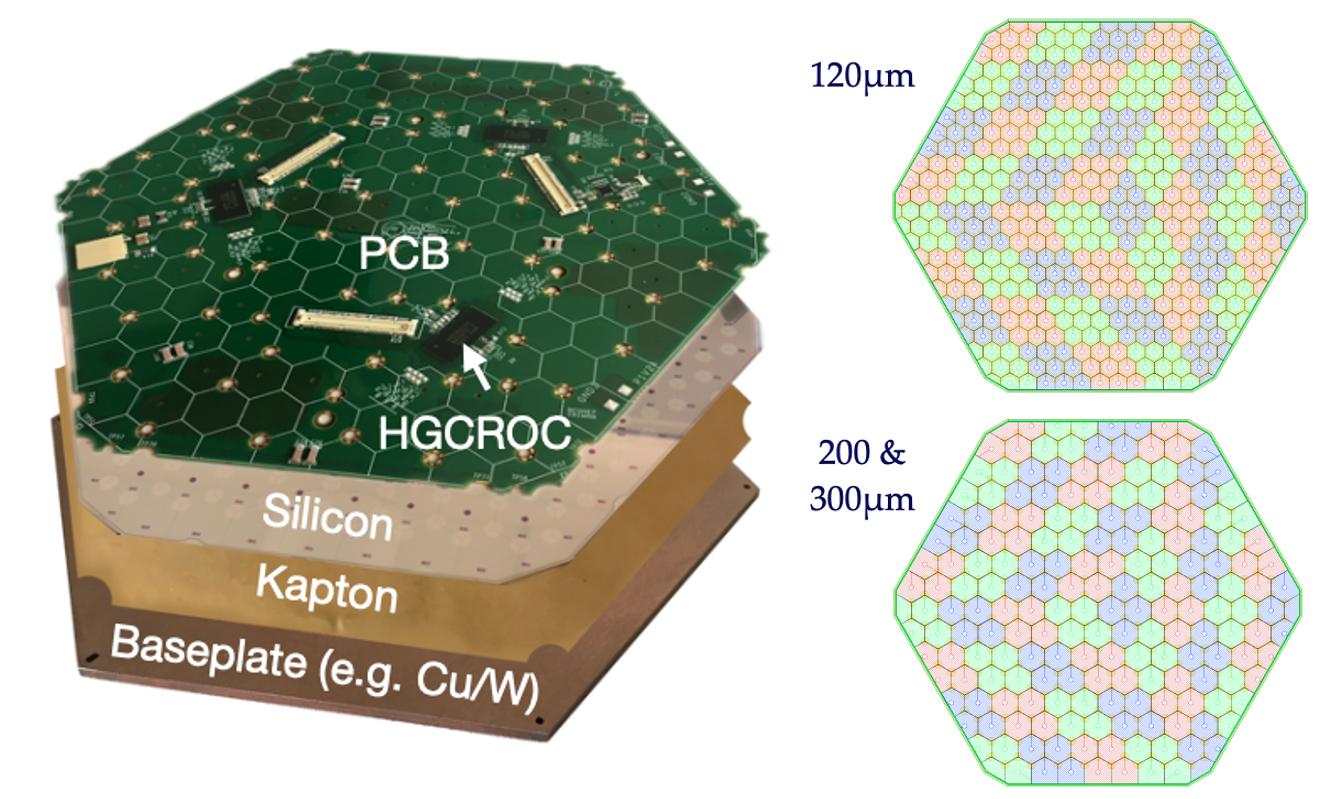
\includegraphics[width=0.7\textwidth]{figures/chapter05/HGCal_layers.jpg}
    \bicaption{\quad \centering 单个HGCal模块结构示意图~\cite{Quast:2791449}}{\quad \centering Schematic diagram of single HGCAL module~\cite{Quast:2791449}}
    \label{fig:c05f02}
\end{figure}

为了应对在HL-LHC阶段中高额的堆积事例,量能器的选择需要具有足够高的颗粒性,可以更加精确的辨别出对撞粒子所产生的簇射分布,同时也可以利用精确的时间测量辨别初级对撞顶点;除此之外,海量的辐射本底也要求探测器模块具有极高的抗辐照性,而HGCal正好具备了以上所有要求。在升级完成后,HGCal可以覆盖CMS探测器$1.5<|\eta|<3.0$的范围,如图~\ref{fig:c05f01}所示,电磁量能器部分(CE-E)是由钨铜板和铅吸收层以及硅传感器交错组成的,一共含有26层;强子量能器部分(CE-H)是由钢吸收层和硅传感器加闪烁体/硅光电倍增管交互组成的,一共含有21层。每个HGCal模块的示意图如图~\ref{fig:c05f02}所示,主要由基础板层(Baseplate)、聚酰亚胺薄膜层(Kapton)、硅片层(Silicon)和印刷电路板层(PCB)构成,其中,Baseplate层是由钨铜板构成的,主要作用是作为吸收层以及为整个模块提供支撑;Kapton层的作用是为Silicon和Baseplate之间提供绝缘层;Silicon层的作用是作为粒子穿过探测器时的激活层;PCB层的作用是将粒子穿过探测器时产生的信号读出。根据不同的区域,HGCal模块所使用的设计不同:在更接近于束流的区域,具有更高的本底辐射强度,因此采用了更薄的硅模块,厚度为120~\si{\um},每个硅模块具有432个读出单元,每个单元面积大约为0.6~\si{\cm^{2}};而在远离束流的区域,具有更高的径迹密度,因此可以采用更高厚度的硅模块,厚度为200~\si{\um}或者300~\si{\um},每个硅模块具有192个读出单元,每个单元的面积大约为1.2~\si{\cm^{2}}。

为了在LHC第三阶段停机过程中将端盖部分的量能器全部替换为HGCal,总共需要生产26000块硅模块。为此,中国科学院高能物理研究所参与并承担了部分HGCal模块的组装生产工作,并建立了相应的模块生产中心,洁净间的俯视图如图~\ref{fig:c05f03}所示,总占地面积大约170~\si{\m^{2}},主要仪器有:Gantry工作平台、OGP工作平台、Wirebonder工作台等,其中Gantry工作平台主要负责对Baseplate、Kapton、Silicon和PCB进行组装粘合;OGP工作平台主要用来对模块进行精确定位测量以及对组装结果进行检验;Wirebonder工作台主要是负责打线,连接PCB板和Silicon。

\begin{figure}[!htbp]
    \centering
    %trim option's parameter order: left bottom right top
    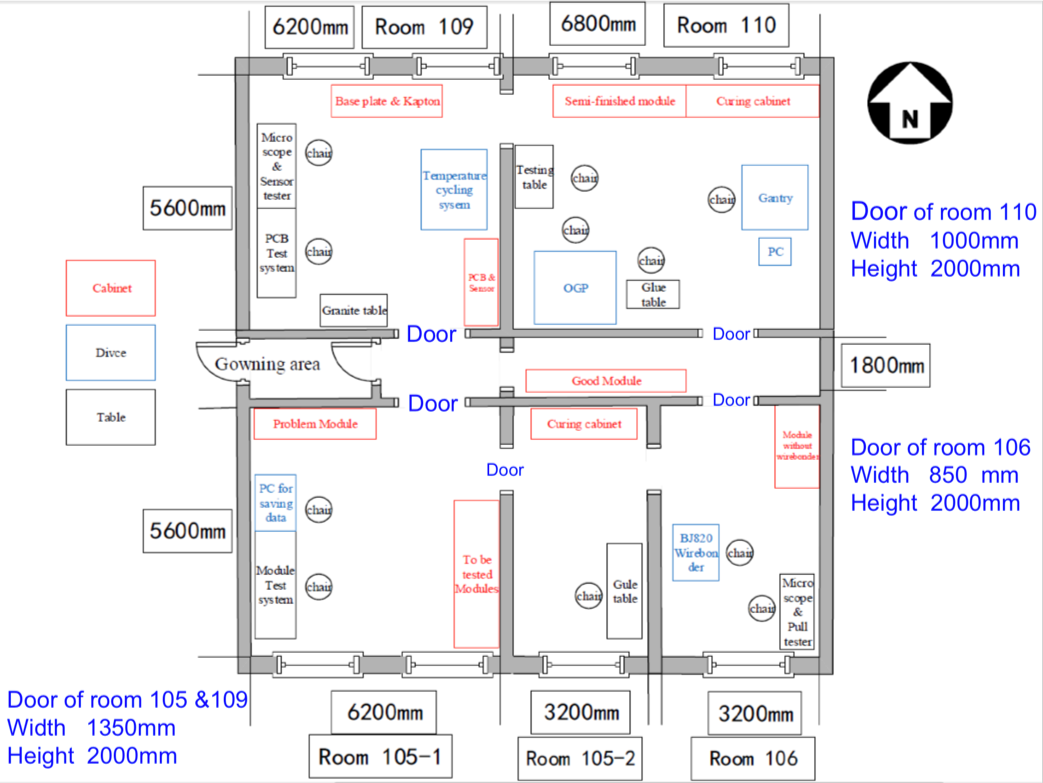
\includegraphics[width=1.0\textwidth]{figures/chapter05/HGClab.png}
    \bicaption{\quad \centering 洁净间平面图}{\quad \centering Clean room floor plan}
    \label{fig:c05f03}
\end{figure}

2021年6月31日,中国科学院高能物理研究所CMS课题组成功完成了8英寸的HGCal模块样机的试制,如图~\ref{fig:c05f04}和图~\ref{fig:c05f05}所示,这是当时CMS合作组第一块使用最新设计的前端电子学NSH HGCROC V2制作的8寸硅模块,也是CMS合作组首次有除美国加州大学圣芭芭拉分校(UCSB)外的单位成功制作高粒度量能器硅模块。本人主要参与了此模块制作过程中使用Gantry工作平台对模块进行组装的部分。

\begin{figure}[!htbp]
    \centering
    %trim option's parameter order: left bottom right top
    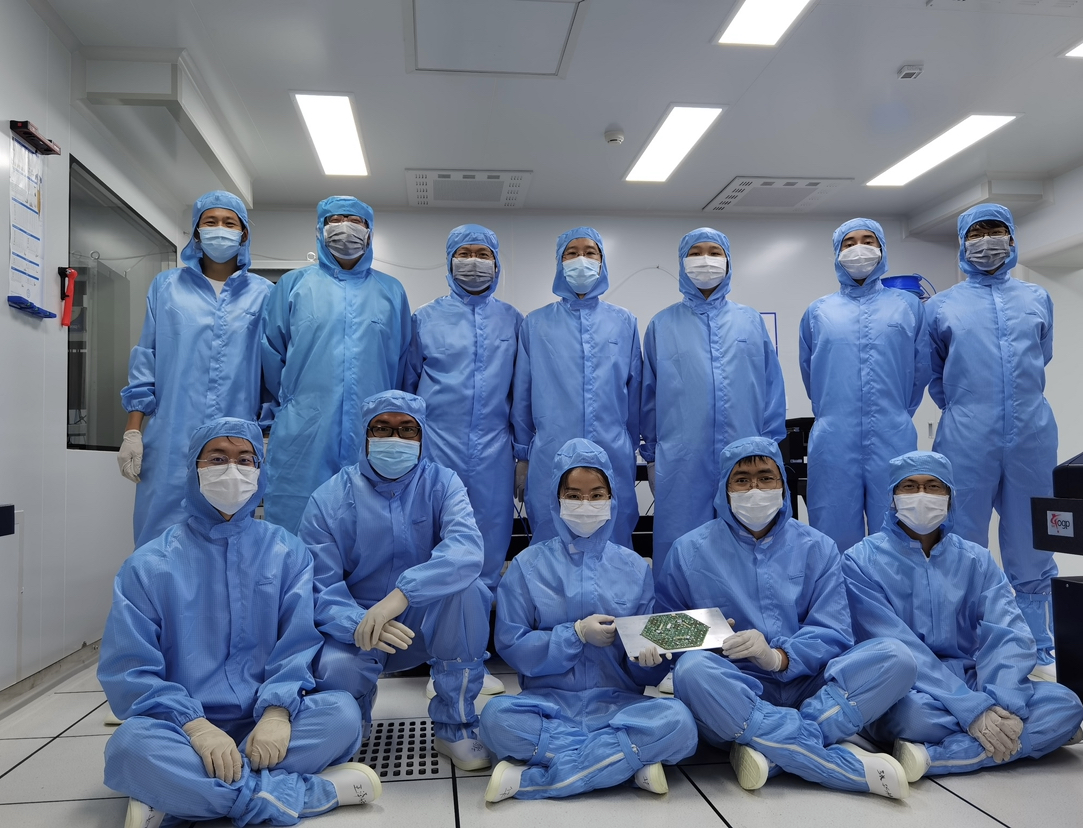
\includegraphics[width=0.7\textwidth]{figures/chapter05/HGCal_group.jpeg}
    \bicaption{\quad \centering 制作8寸模块的部分团队成员合影}{\quad \centering The group photo for part of the group member, who made the 8-inch HGCal module}
    \label{fig:c05f04}
\end{figure}

\begin{figure}[!htbp]
    \centering
    %trim option's parameter order: left bottom right top
    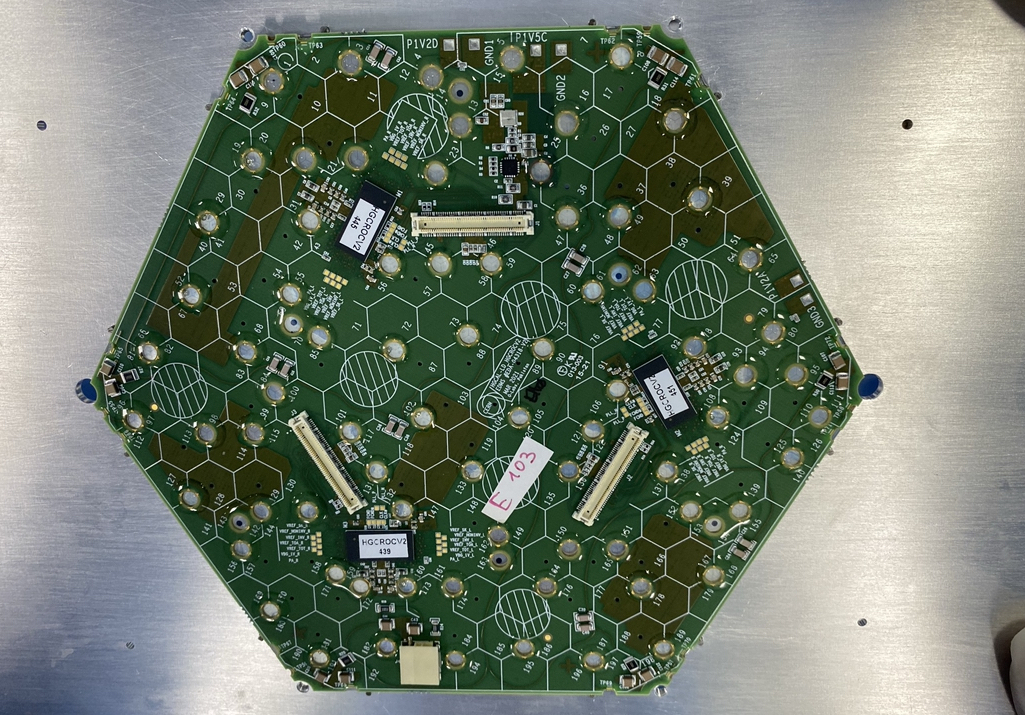
\includegraphics[width=0.5\textwidth]{figures/chapter05/HGCal_sample.jpeg}
    \bicaption{\quad \centering 首块8英寸HGCal模块}{\quad \centering First 8-inch HGCal module}
    \label{fig:c05f05}
\end{figure}

图~\ref{fig:c05f06}展示了Gantry工作平台的外观图,它主要由一个可以横向和纵向移动的悬臂、负责摆放组装所需工装的平台、一个可以垂直方向移动并且负责抓取模块的Gantry Head以及真空系统所组成,它的组装精度可以达到微米级别,是国内目前唯一一台高精度、大量程的Gantry工作平台。模块组装步骤如下:
\begin{itemize}
    \item 首先,将粘好Kapton的Baseplate和Silicon放置在工作平台的工装上;
    \item 然后,利用Gantry Head将胶管定位到Kapton上,向胶管中添加胶水并准备点胶;
    \item 启动点胶程序,在Kapton上完成第一层点胶,并将胶管取下;
    \item 将Gantry Head定位到放置Silicon的工装上,利用真空系统抓取Silicon并将其粘贴到Kapton上;
    \item 将Gantry Head定位到胶水厚度控制的工装上,抓取工装并将其放置在粘好Silicon的Baseplate上,等待胶水凝固;
    \item 胶水凝固后将厚度控制的工装移除,将PCB板放置到工装上准备安装;
    \item 同第一层点胶步骤一样,在Silicon上进行第二层点胶;
    \item 而后,利用Gantry Head抓取PCB板,并将其放置到Silicon上,等待胶水凝固,组装完成。
\end{itemize}

\begin{figure}[!htbp]
    \centering
    %trim option's parameter order: left bottom right top
    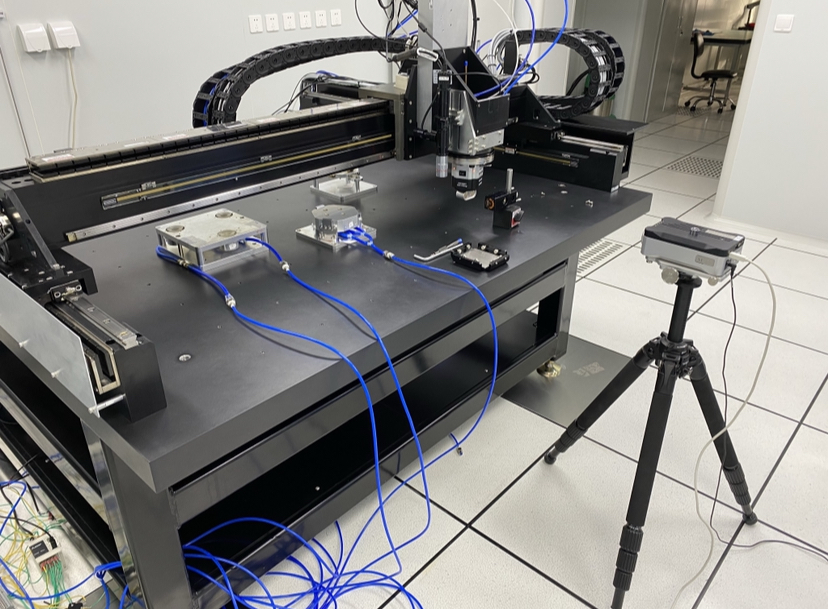
\includegraphics[width=1.0\textwidth]{figures/chapter05/Gantry.jpeg}
    \bicaption{\quad \centering Gantry工作平台外观图}{\quad \centering Appearance of Gantry working platform}
    \label{fig:c05f06}
\end{figure}

以上组装步骤中一共需要进行两次点胶操作,但是,由于两次点胶的基准面不同,点胶模式也有所不同,如图~\ref{fig:c05f07}所示。对于在Kapton上的点胶模式,由于Silicon和Kapton之间属于无缝隙粘贴,因此点胶模式选择了和Baseplate形状相同的正六边形模式
。而对于Silicon上的点胶模式,由于PCB板上具有特定的镂空圆孔结构,这些结构是为了组装完成后进行bonding,从而连接PCB板和Silicon的,因此在Silicon上的第二层点胶路径需要绕过这些用于Bounding的位置,于是本团队采取了在对应的Bounding位置附近使用圆形或者半圆形的点胶路径。本人负责了第二层点胶路径的设计,设计结果如图~\ref{fig:c05f08}所示。

\begin{figure}[!htbp]
    \centering
    %trim option's parameter order: left bottom right top
    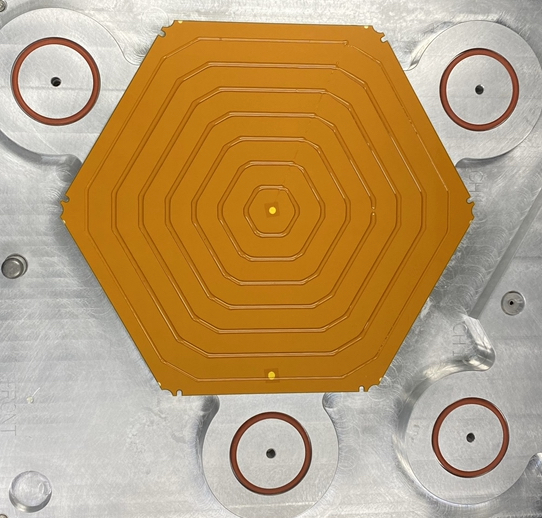
\includegraphics[width=0.4\textwidth]{figures/chapter05/Dispensing_first.jpeg}
    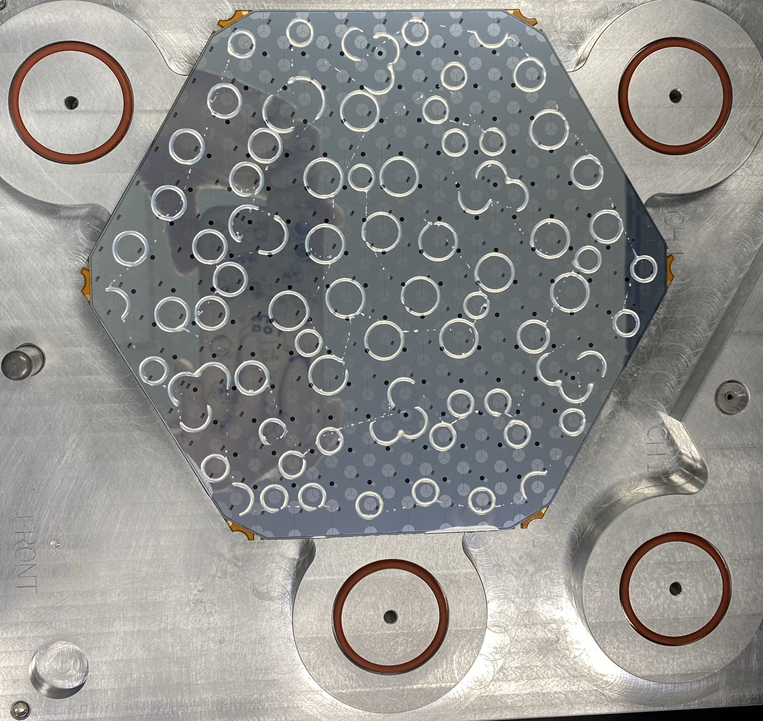
\includegraphics[width=0.4\textwidth]{figures/chapter05/Dispensing_second.jpeg}
    \bicaption{\quad \centering 第一层(左图)和第二层(右图)点胶模式}{\quad \centering Dispensing modes for the first (left) and second (right) layers}
    \label{fig:c05f07}
\end{figure}

\begin{figure}[!htbp]
    \centering
    %trim option's parameter order: left bottom right top
    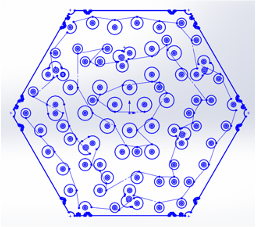
\includegraphics[width=0.5\textwidth]{figures/chapter05/Dispensing_2nd_path.png}
    \bicaption{\quad \centering 第二层点胶模式设计}{\quad \centering Dispensing modes design for the second layer}
    \label{fig:c05f08}
\end{figure}

\begin{figure}[!htbp]
    \centering
    %trim option's parameter order: left bottom right top
    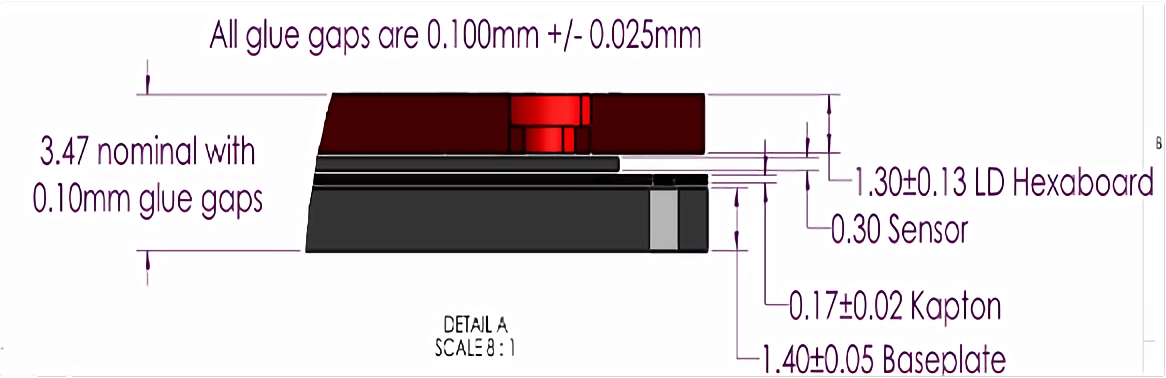
\includegraphics[width=1.0\textwidth]{figures/chapter05/glue.png}
    \bicaption{\quad \centering HGCal模块胶水厚度控制}{\quad \centering HGCal module glue thickness control}
    \label{fig:c05f09}
\end{figure}

在安装完成后,需要对模块进行厚度测试,原因是在最终的探测器安装过程中,需要考虑模块厚度对最终安装的影响,而各个模块部分的厚度是一定的,因此对模块厚度的控制最终就体现到了对两层胶水厚度的控制。图~\ref{fig:c05f09}展示了HGCal模块组装过程中所需的胶水厚度控制示意图,组装模块时所使用的胶水层厚度必须被严格控制在$100\pm25~\si{\um}$的范围内。因此,如何控制好胶水的厚度是成功组装模块的关键。为此,本团队对工装进行了水平校准,使得组装平台的四个角在垂直方向上的误差小于25~\si{\um},Gantry Head的水平误差在8~\si{\um}左右,最终胶水的厚度测量结果为$103\pm15~\si{\um}$,满足HGCal模块的生产要求,成功生产出当时第一块8英寸的HGCal模块。

\section{CSC探测器寿命研究}

CSC探测器全称阴极条形室(Cathode Strip Chambers),是CMS实验中端盖缪子探测器的一部分,主要作用是测量缪子径迹。CSC探测器的结构在第~\ref{sec:MuonDetector}节已经有过介绍。目前为止,运行在CMS实验上的CSC探测器中的气体是由40\%的$\mathrm{Ar}$、50\%的$\mathrm{CO_2}$和10\%的$\CF$所组成的。其中,$\mathrm{CO_2}$占据了绝大多数成分,它的主要作用是作为不易燃的淬火气体,可以通过吸收光子最大限度地减少杂散脉冲,从而有助于探测器的稳定运行;而$\CF$本身也是一种淬火气体,但是引入$\CF$作为气体成分的最初目的是可以防止丝室发生老化,影响探测器的使用寿命;$\mathrm{Ar}$的作用是降低探测器的工作电压。

在CSC探测器所使用的气体中,$\CF$作为一种非常重要的气体,可以有效的防止探测器发生老化,但是与此同时,高额的气体费用和使用$\CF$所带来的温室效应使得减少此气体的使用作为未来探测器发展所必需的一环。图~\ref{fig:c05f10}展示了目前应用在CMS实验CSC探测器上的$\CF$气体回收系统,这个系统从2012年开始运行,到目前为止一共回收了大约450~\si{\m^{3}}的$\CF$气体,减少了大约44\%的温室气体排放,目前对$\CF$的回收效率大概在50\%--70\%之间。CERN承诺,要在Run5开始正式取数之前将温室气体的排放相比于2016年的水平降低70\%,而CERN所排放的温室气体中超过78\%的气体是含氟气体,因此寻找降低CSC探测器中$\CF$气体使用的方案成为了重中之重。目前CMS实验CSC课题组主要考虑了以下两种方案:
\begin{itemize}
    \item 降低CSC探测器使用的气体中$\CF$的含量;
    \item 寻找$\CF$的替代品,选择温室效应影响更低的气体。
\end{itemize}

\begin{figure}[!htbp]
    \centering
    %trim option's parameter order: left bottom right top
    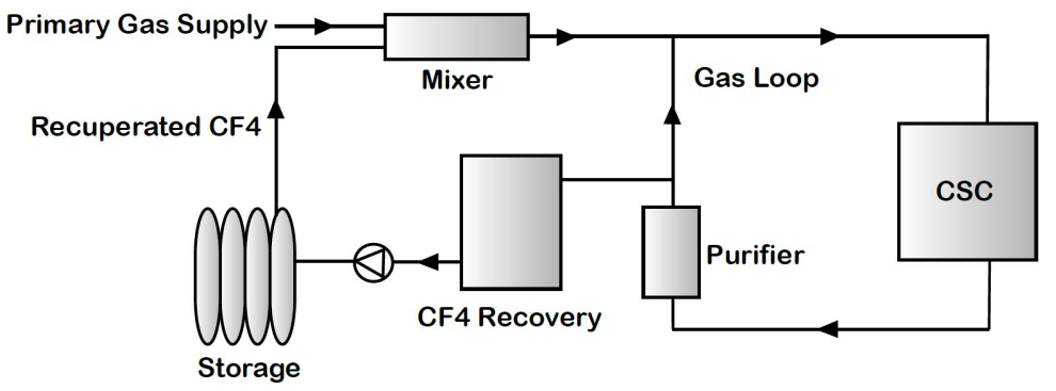
\includegraphics[width=1.0\textwidth]{figures/chapter05/CSC_CF4_recuperation.png}
    \bicaption{\quad \centering CMS CSC探测器$\CF$气体回收系统~\cite{CSCGas}}{\quad \centering $\CF$ gas recuperation systems for CMS CSC~\cite{CSCGas}}
    \label{fig:c05f10}
\end{figure}

对于第一种方案,我们考虑了将$\CF$的含量降低到2\%,但是由于$\CF$的作用是防止探测器发生老化,降低它的含量有可能对探测器产生损坏。因此,研究CSC探测器在不同气体成分条件下的使用寿命对降低所用气体中$\CF$的含量具有重要的意义。

为此,我们对两个全尺寸的CSC探测器在$\CF$成分为2\%的气体组成条件下进行了研究,所使用的两个CSC探测器分别标记为ME1/1和ME2/1,它们是目前运行在CMS实验上的两种CSC探测器,其中ME1/1相比于ME2/1具有更小的尺寸,原因是由于靠内的探测器处于磁场更强的环境中。当缪子穿过探测器时,电离所产生的电子和阳离子在电场的作用下会分别向阳极丝和阴极板所移动,同时在磁场的作用下,它们的移动轨迹会发生偏转,进而使得缪子轨迹的分辨率和探测效率降低,但是尺寸较小的探测器具有更短的漂移距离,由磁场所引发的轨迹偏转会更小,从而使得尺寸较小的CSC探测器可以在靠近内部的位置相比于尺寸较大的探测器获得更好的空间分辨率和探测效率。

根据计算,由于LHC对撞时产生的高量辐射,ME1/1类型的CSC探测器在HL-LHC阶段总共会累积大约0.2~\si{{\coulomb\per\cm}}的电荷量,ME2/1类型的CSC探测器会累积大约0.13~\si{{\coulomb\per\cm}}的电荷量。为了模拟改变气体成分后的CSC探测器在高辐射背景下的探测器使用寿命,我们将这两个CSC探测器放置在了伽马辐照设施GIF++中进行测试。

\begin{figure}[!htbp]
    \centering
    %trim option's parameter order: left bottom right top
    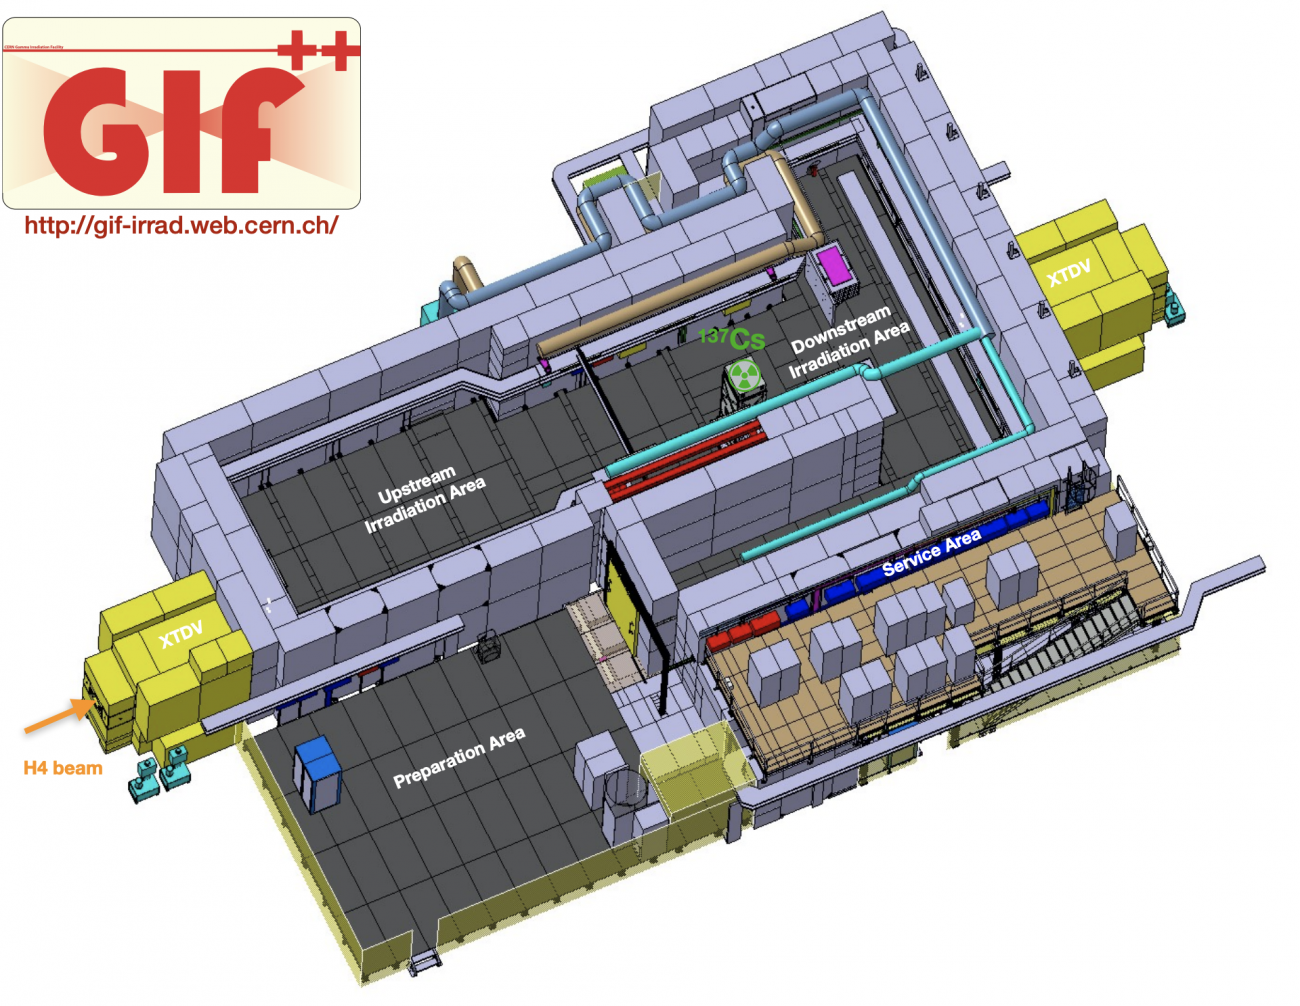
\includegraphics[width=1.0\textwidth]{figures/chapter05/GIF_layout.png}
    \bicaption{\quad \centering 伽马辐照设施GIF++的布局~\cite{gif}}{\quad \centering The layout of Gamma Irradiation Facility GIF++~\cite{gif}}
    \label{fig:c05f11}
\end{figure}

GIF++的全称是Gamma Irradiation Facility,它是位于欧洲核子研究中心Prévessin园区的一个束流测试设备,可以用于测试和评定高能物理实验、太空任务和其他辐射敏感应用中使用的各种电子元件、传感器和探测器的辐射硬度。GIF++设施的布局如图~\ref{fig:c05f11}所示,占地面积大约为100~\si{\m^{2}},包括一个高强度的$^{137}\mathrm{Cs}$伽马源,可以产生能量范围从10~\si{\keV}到15~\si{\MeV}的伽马射线,是世界上最高强度的伽马辐照设施之一。除此之外,GIF++还位于SPS的束流管道之上,因此可以同时接收由SPS传递过来的高能带电粒子束流,这些束流的能量在10$\GeV$到450$\GeV$之间,通过轰击T2靶目标可以产生能量小于150$\GeV$的缪子束流,进而可以对放置在其中的探测器进行缪子束流测试。为了防止辐射泄漏,整个设施都处于厚度为1.6米的混凝土墙掩体内。由于伽马源和SPS是相互独立的,因此原则上可以全年运行伽马源,对处于其辐射范围内的探测器进行高辐射模拟。在经历一段时间的辐射后,可以转为缪子模式,研究辐射对探测器缪子重建效率的影响。

\begin{figure}[!htbp]
    \centering
    %trim option's parameter order: left bottom right top
    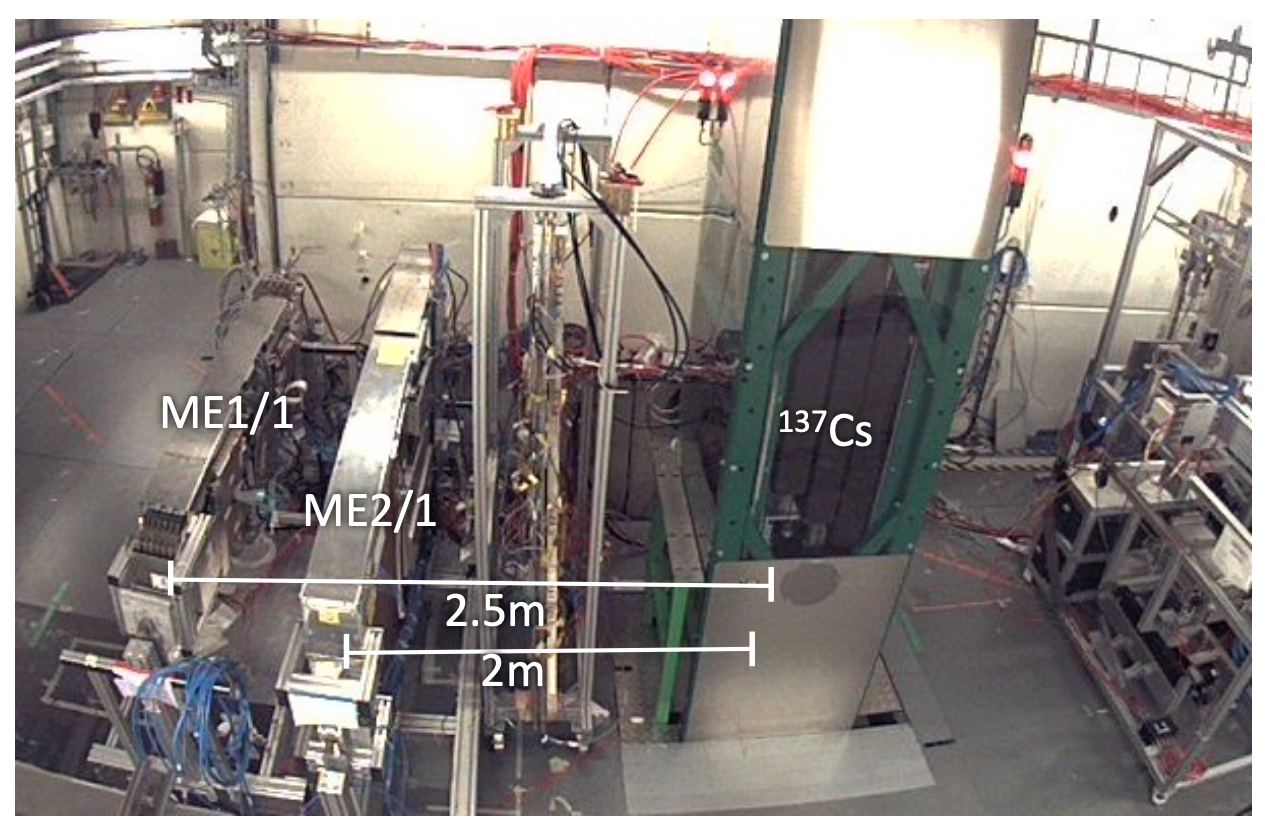
\includegraphics[width=0.7\textwidth]{figures/chapter05/GIF_CSC.jpg}
    \bicaption{\quad \centering GIF++的设置,其中展示了ME1/1和ME2/1相对于$\mathrm{^{137}Cs}$伽马源的辐射位置}{\quad \centering Setup of GIF++, which shows the irradiation position for ME1/1 and ME2/1 relative to the $\mathrm{^{137}Cs}$ gamma source}
    \label{fig:c05f12}
\end{figure}

CSC探测器的寿命研究开始于2016年,两个探测器在GIF++中的位置如图~\ref{fig:c05f12}所示,其中ME1/1距辐射源2.5~\si{\m},ME2/1距辐射源2~\si{\m}。为了模拟HL-LHC中的辐射本底,到目前为止,两个CSC探测器一共累积了0.7~\si{{\coulomb\per\cm}}的电荷量。其中,对于$\CF$的含量为10\%的情况,ME1/1和ME2/1分别累积了0.33~\si{{\coulomb\per\cm}}的电荷量,而对于$\CF$的含量为2\%的情况,ME1/1累积了0.37~\si{{\coulomb\per\cm}}的电荷量。在电荷累积的过程中,我们对探测器的性能进行了持续监测,用于研究探测器的使用寿命。对探测器性能的测量主要包括Dark rate测量和Strip to strip电阻测量这两种方法,详细研究方法会在第~\ref{sec:darkrate}节和第~\ref{sec:s2s}节进行介绍。研究结果表明,对于$\CF$含量为2\%的混合气体,并没有观测到探测器发生明显的性能下降。但是,通过对不同$\CF$含量下的阳极丝表面进行观测可以发现,2\%的$\CF$含量会使得阳极丝表面产生肉眼可见的沉积,如图~\ref{fig:c05f13}所示。因此,我们认为将$\CF$的含量降低至2\%可能是存在一定风险的,5\%的$\CF$含量应该是比较好的选择。为此,现在正在进行的测量是基于5\%的$\CF$,希望可以在未来的测量中证实5\%的$\CF$可以应用到实际的CMS实验中。

\begin{figure}[!htbp]
    \centering
    %trim option's parameter order: left bottom right top
    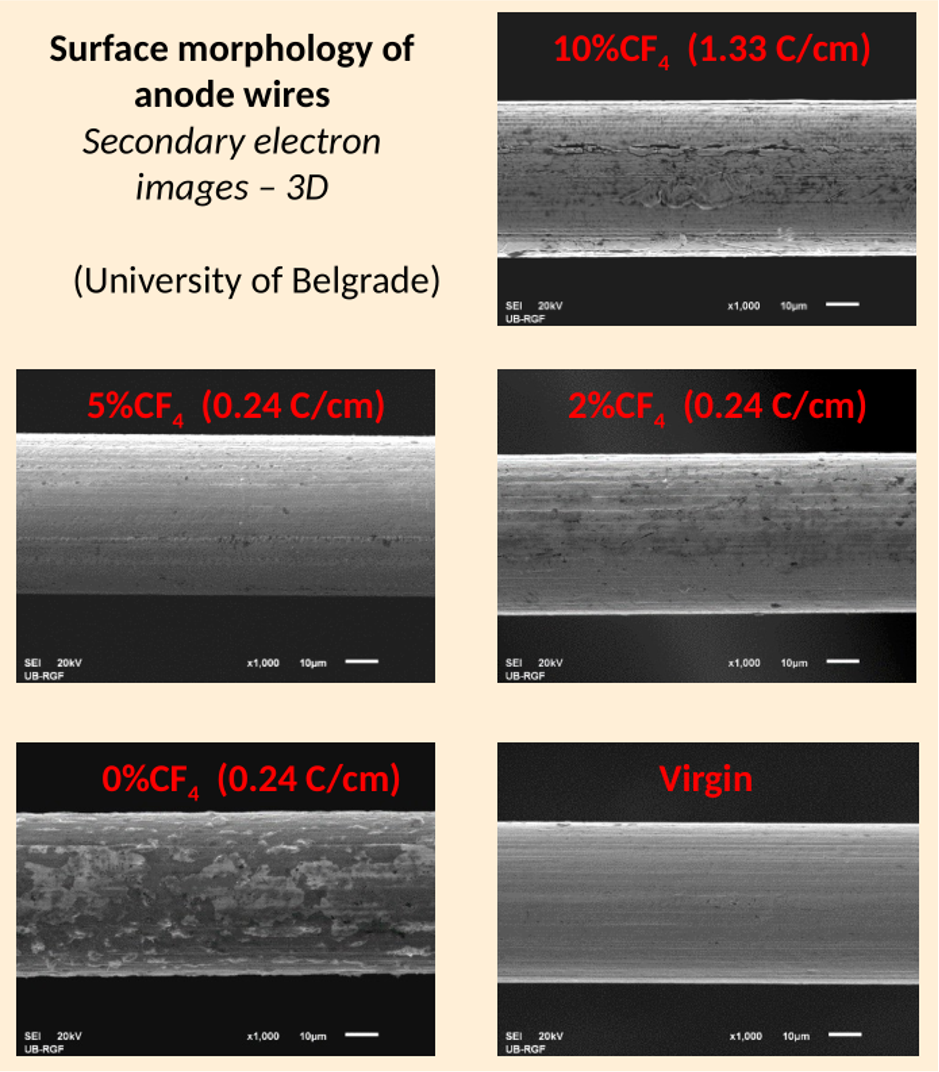
\includegraphics[width=0.7\textwidth]{figures/chapter05/CSC_deposit.png}
    \bicaption{\quad \centering 10\%、5\%、2\%和0\%$\CF$快速辐照试验下阳极丝表面的显微图}{\quad \centering Microscopic view of the anode wire surfaces under the fast irradiation test with 10\%, 5\%, 2\%, and 0\% $\CF$}
    \label{fig:c05f13}
\end{figure}

而对于第二种方案,我们也尝试着将$\CF$替换为温室效应更低的气体,比如HFO1234ze气体。这种气体相对于二氧化碳的全球变暖潜势(Global Warming Potentials)小于1,而$\CF$相对于二氧化碳的全球变暖潜势大约为6400。为此,我们在实验室构建了MiniCSC原型,这是专为这项研究所构建的小型CSC探测器,它的结构如图~\ref{fig:c05f14}所示。它由三个面板所构成,形成两个气体间隙,构建MiniCSC所使用的材料和电子学与运行在CMS实验上正常尺寸的CSC探测器相同。目前,我们一共构建了6块MiniCSC,利用这些原型机可以进行快速的性能测试和辐照测试。为了研究不同气体成分下CSC探测器的性能,我们在实验室也构建了相应的动态气体混合系统,如图~\ref{fig:c05f15}所示,左图为气体混合器,右图为气体气缸和压力调节阀。

\begin{figure}[!htbp]
    \centering
    %trim option's parameter order: left bottom right top
    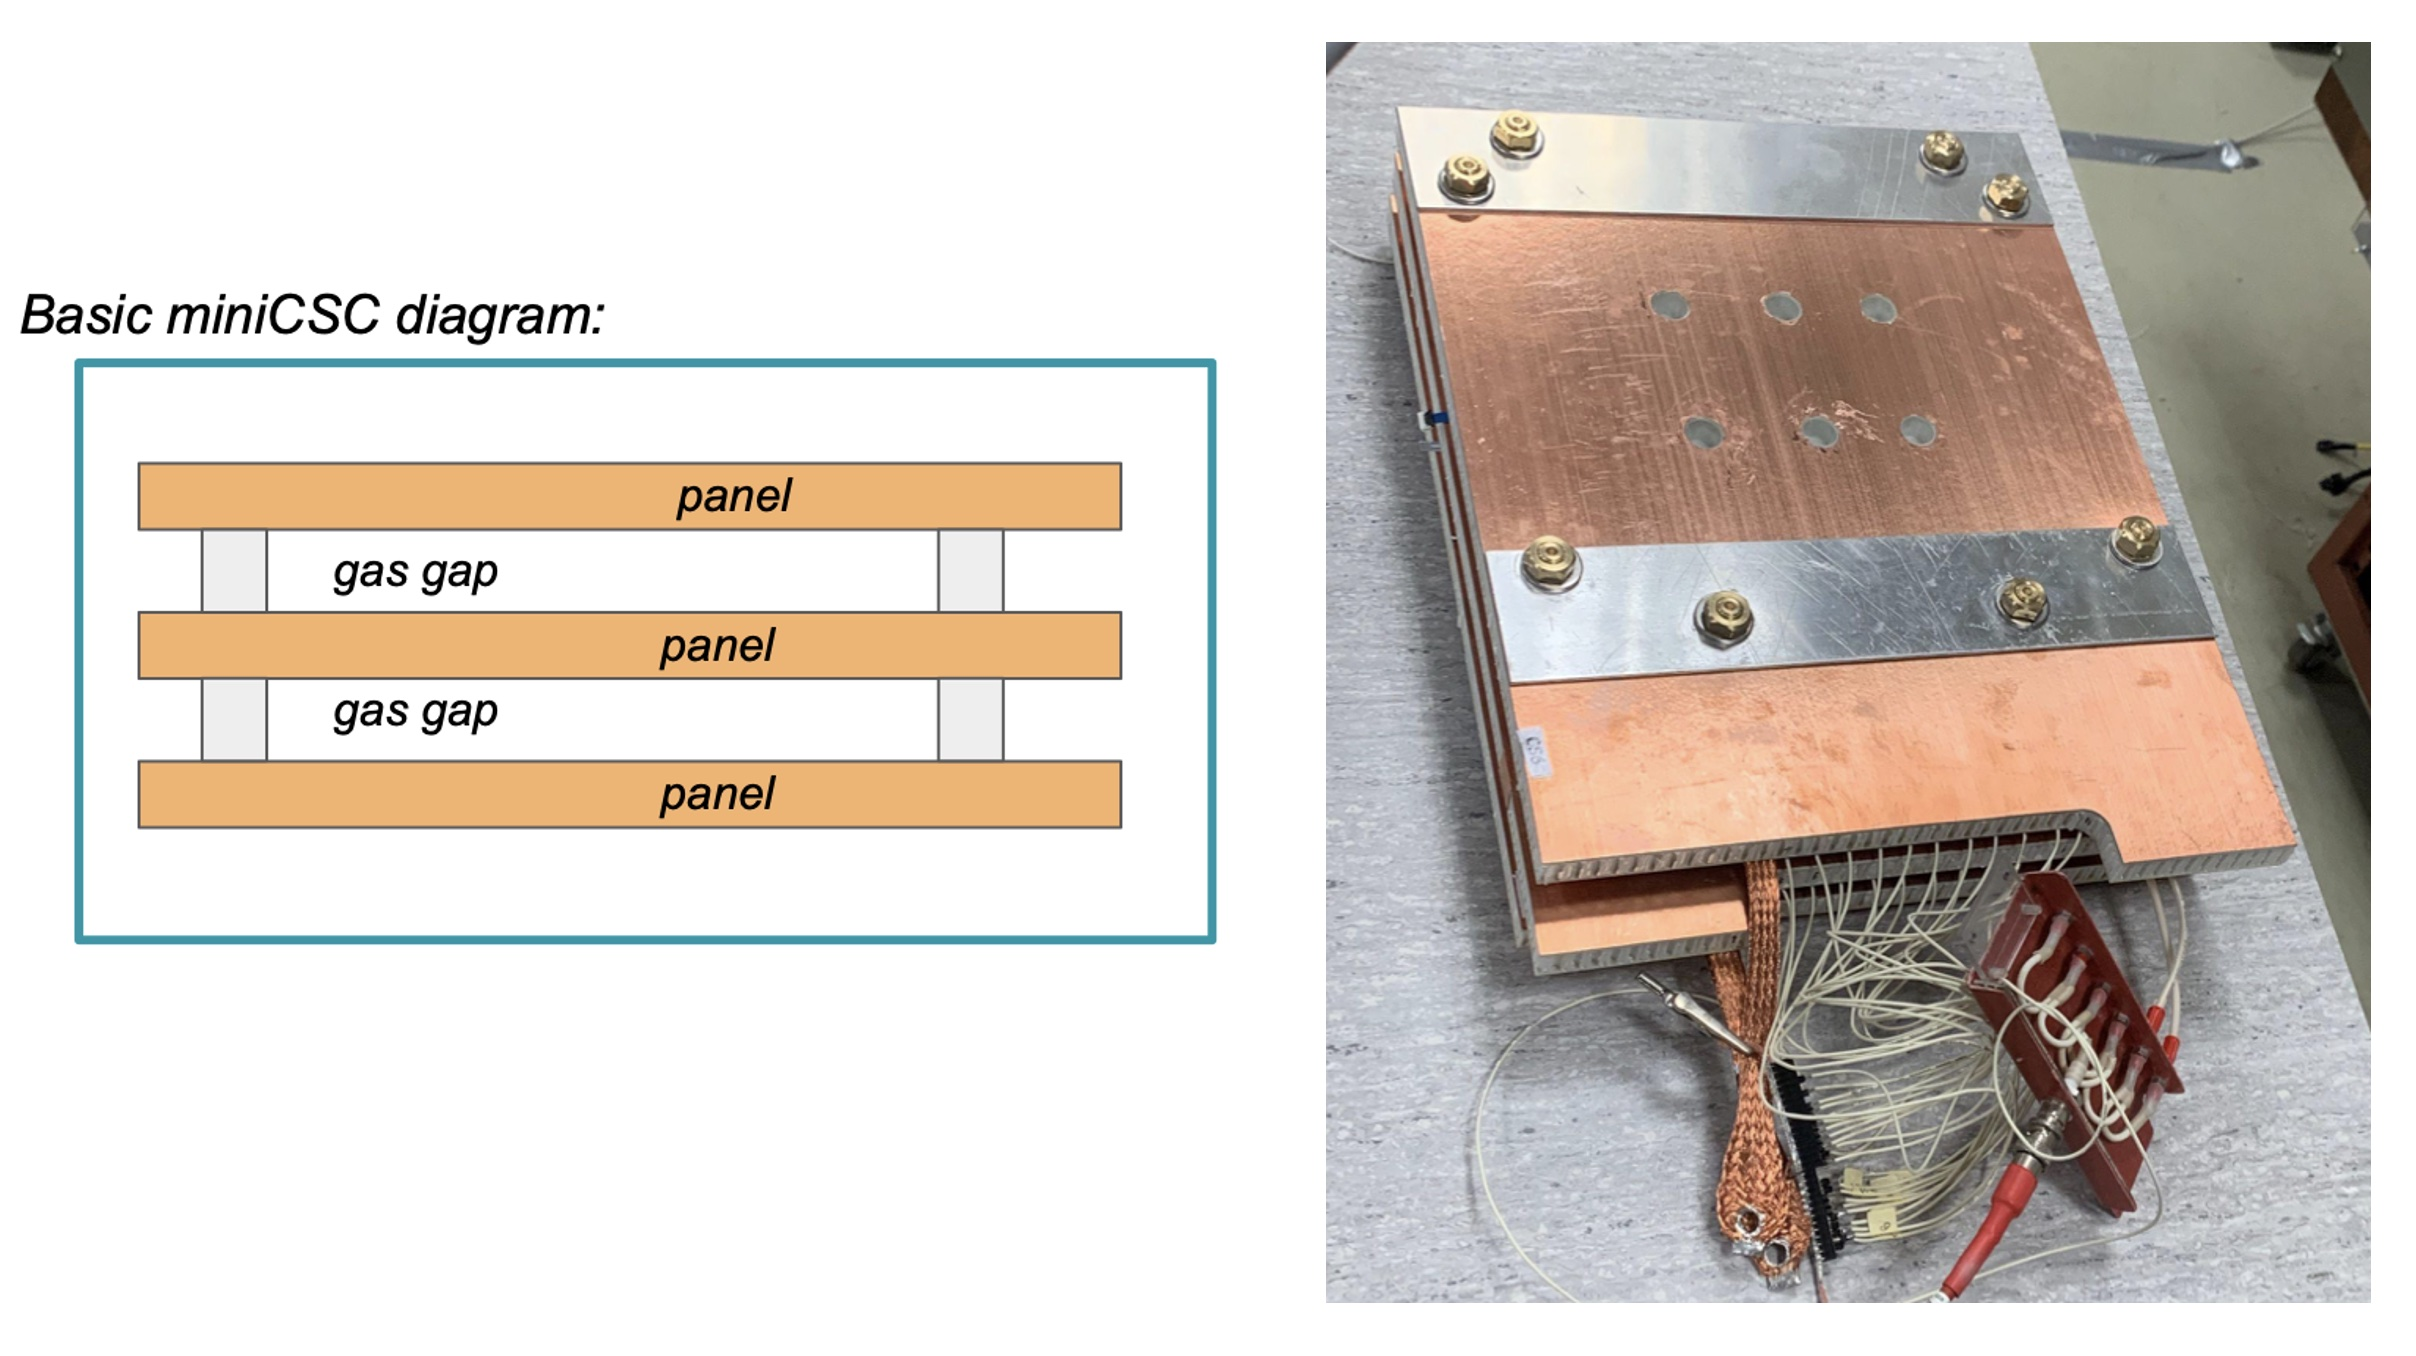
\includegraphics[width=0.7\textwidth]{figures/chapter05/MiniCSC.jpg}
    \bicaption{\quad \centering MiniCSC结构示意图}{\quad \centering Schematic diagram of MiniCSC structure}
    \label{fig:c05f14}
\end{figure}

\begin{figure}[!htbp]
    \centering
    %trim option's parameter order: left bottom right top
    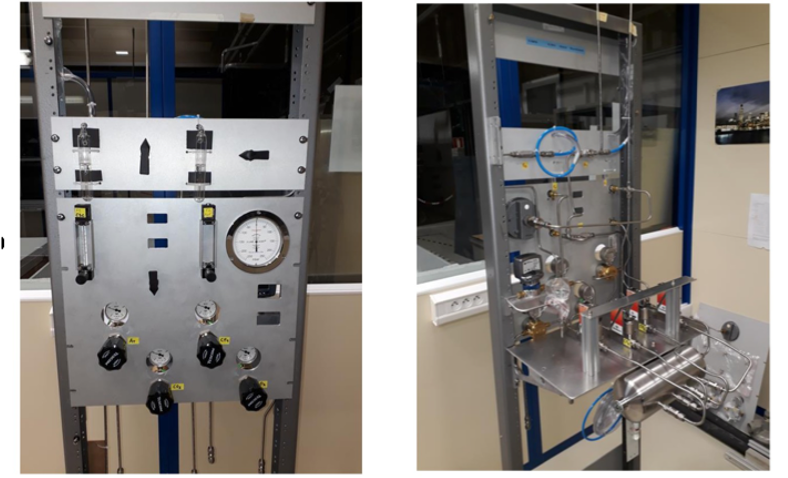
\includegraphics[width=0.7\textwidth]{figures/chapter05/MiniCSC_GasMixer.png}
    \bicaption{\quad \centering MiniCSC动态气体混合系统}{\quad \centering Dynamic mixing gas system for MiniCSC}
    \label{fig:c05f15}
\end{figure}

在对MiniCSC的测量过程中,冲入的混合气体成分为40\%的氩气、58\%的二氧化碳和2\%的HFO1234ze气体。图~\ref{fig:c05f16}展示了MiniCSC的阳极丝中暗电流的测量作为累积电荷的函数,可以发现,对于受到辐照的阳极丝,暗电流有了显著的增长,并且这个现象仅在使用HFO1234ze作为混合气体的情况下被观测到。除此之外,我们也在辐照后的阳极丝表面观察到了显著的氧化钨沉积,如图~\ref{fig:c05f17}所示。这些结果表明HFO1234ze气体目前还不能够完全替代$\CF$,需要在未来对其进行更加深入的研究。

\begin{figure}[!htbp]
    \centering
    %trim option's parameter order: left bottom right top
    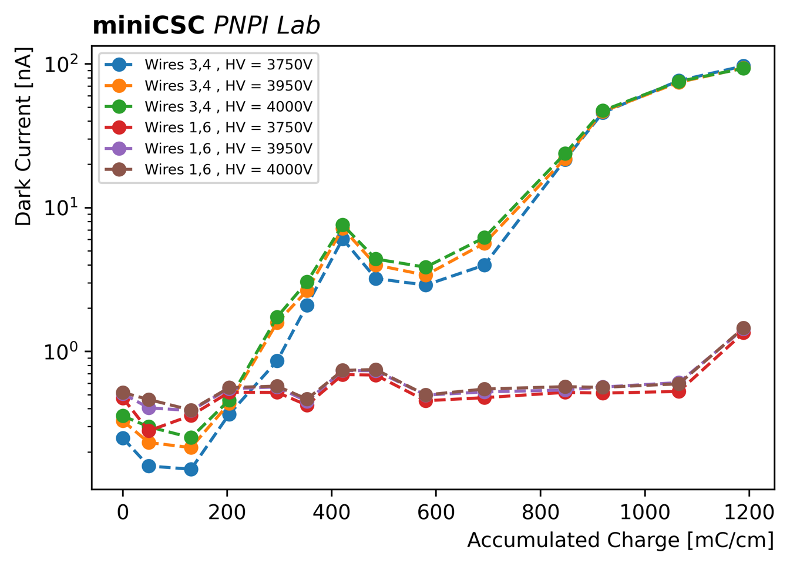
\includegraphics[width=0.7\textwidth]{figures/chapter05/MiniCSC_darkcurrent.png}
    \bicaption{\quad \centering MiniCSC的阳极丝暗电流测量作为累积电荷的函数}{\quad \centering Anode-wire dark current measurements for MiniCSC as a function of the accumulated charge}
    \label{fig:c05f16}
\end{figure}

\begin{figure}[!htbp]
    \centering
    %trim option's parameter order: left bottom right top
    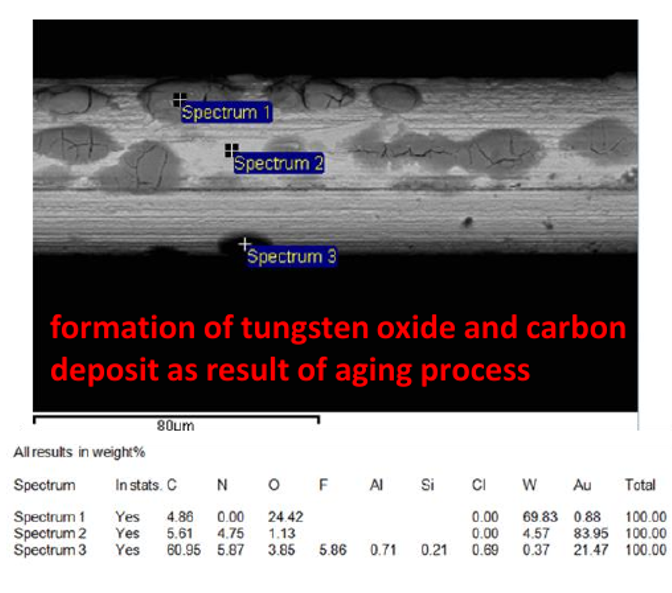
\includegraphics[width=0.5\textwidth]{figures/chapter05/MiniCSC_deposit.png}
    \bicaption{\quad \centering 从使用2\%HFO1234ze作为混合气体的MiniCSC辐照区域提取的阳极丝的显微镜视图}{\quad \centering Microscopic view of the anode wire extracted from the irradiation area of the miniCSC irradiated with 2\% HFO1234ze}
    \label{fig:c05f17}
\end{figure}

\subsection{Dark rate测量}\label{sec:darkrate}

\begin{figure}[!htbp]
    \centering
    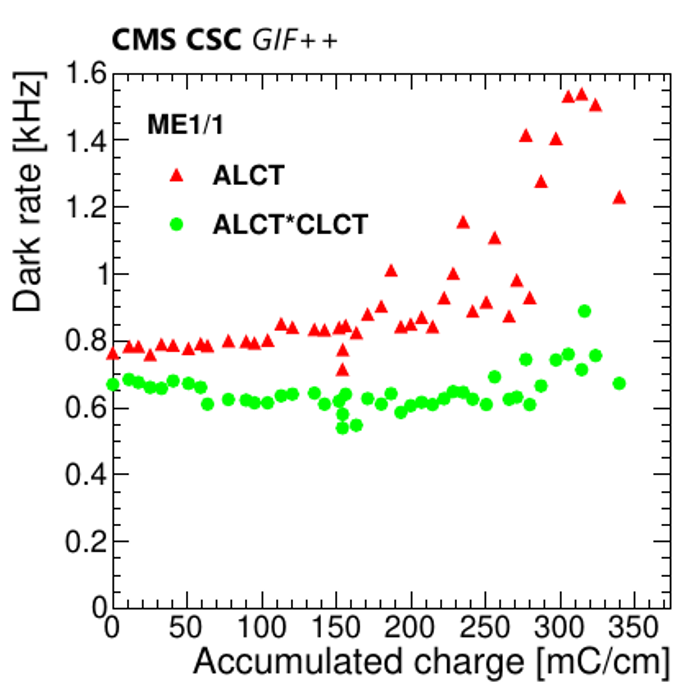
\includegraphics[width=0.35\textwidth]{figures/chapter05/DarkRate_10.png}
    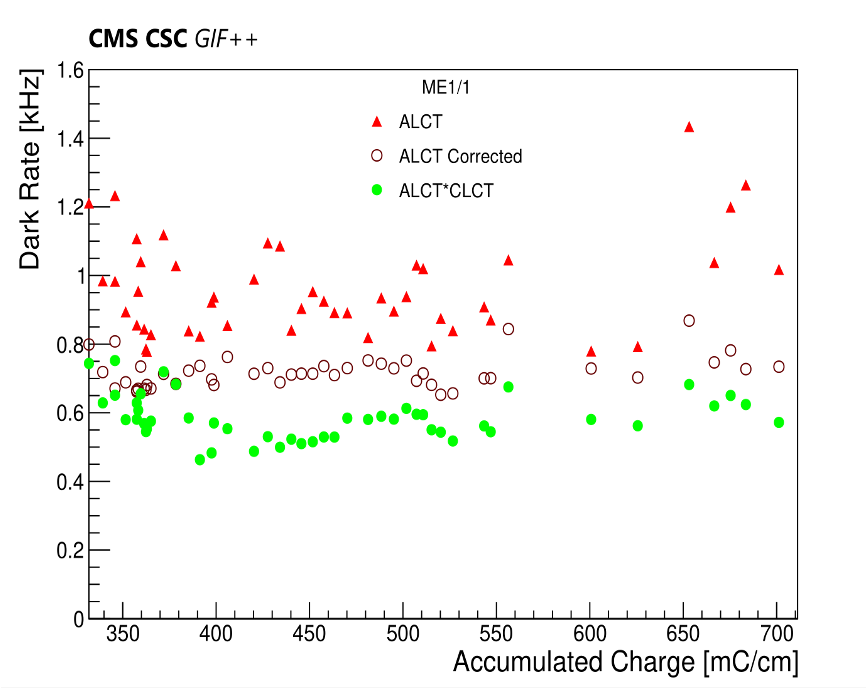
\includegraphics[width=0.45\textwidth]{figures/chapter05/DarkRate_2.png}
    \bicaption{\quad \centering 在10\%的$\CF$(左)和2\%的$\CF$(右)辐照期间测量的 ME1/1 Dark rate作为累积电荷的函数}{\quad \centering ME1/1 dark rate measured during irradiation with 10\% $\CF$ (left) and 2\% $\CF$ (right) as a function of the accumulated charge}
    \label{fig:c05f18}
\end{figure}

Dark rate指的是在没有任何真实粒子信号的情况下,探测器产生噪声信号的比率。Dark rate的测量结果对探测器中阳极丝的老化非常敏感,原因是阳极丝发生老化时会在丝的表面产生沉积,这些沉积会导致丝的表面出现尖锐的不均匀性,在强电场下,这些不均匀的沉积点会产生非常高的电场梯度,更容易引发气体分子中的偶极子,从而使得偶极子的负端被阳极丝所吸引,进而使得Dark rate的测量结果偏高。通过观测CSC探测器的Dark rate作为累积电荷的函数可以得到探测器寿命随着辐照强度增强的影响。图~\ref{fig:c05f18}展示了ME1/1的测量结果,我们记录了10秒的电子学计数,其中左图展示了气体中$\CF$的含量为10\%的测量结果,右图展示了气体中$\CF$的含量为2\%的测量结果。图中红色的点指的是仅通过阳极丝的信号读出系统得出的Dark rate,绿色的点指的是通过配对阳极信号和阴极信号后得出的Dark rate。经比较可以发现,将$\CF$的含量降低至2\%并没有观察到Dark rate发生明显的变化。

\subsection{Strip to strip电阻测量}\label{sec:s2s}

Strip to strip电阻测量是用来测量三组阳极丝两两之间的电阻率的。当沉积物在阳极丝表面形成时,相应的会使得阳极丝的电阻率增大,因此可以通过测量阳极丝之间的电阻率来对探测器的寿命进行监测。具体测量步骤如下:
\begin{itemize}
    \item 首先将电压设置为0~\si{\V},等待6分钟,用于测量本底电阻率;
    \item 然后将电压设置为300~\si{\V},等待7分钟。在这个过程中,测量得到的电流会呈现下降的趋势,而后会逐渐趋于稳定,如图~\ref{fig:c05f19}所示;
    \item 最后将电压调回0~\si{\V},等待6分钟,使得电流稳定。
\end{itemize}
通过拟合可以得到电压稳定在300~\si{\V}和0~\si{\V}的电流值,然后通过计算可以得到对应的电阻率。图~\ref{fig:c05f20}展示了$\CF$含量为2\%的ME1/1的电阻率测量结果,其中不同颜色的点表示不同层之间的测量结果。由此可以看出,将$\CF$的含量降低至2\%并没有使得CSC探测器的电阻测量产生明显的变化。

\begin{figure}[!htbp]
    \centering
    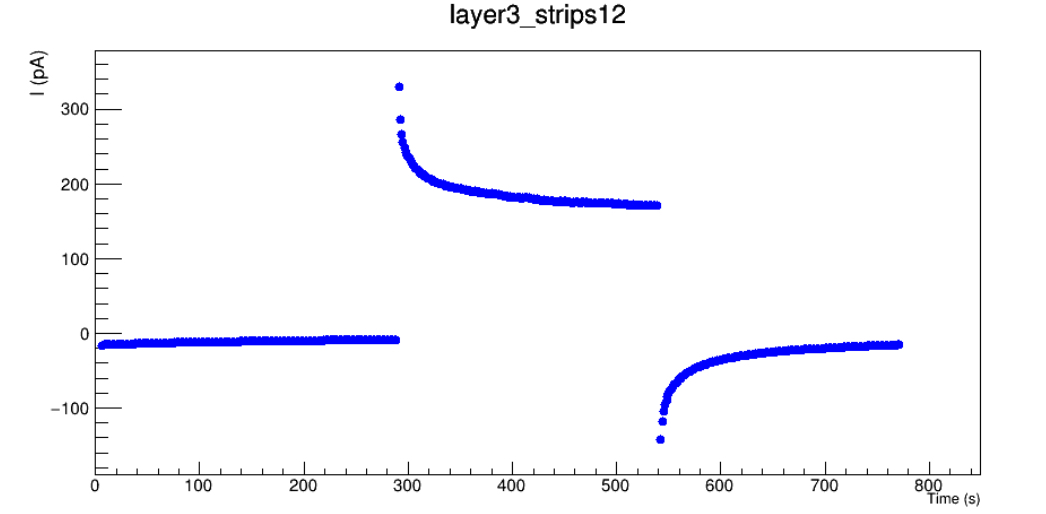
\includegraphics[width=0.8\textwidth]{figures/chapter05/s2s_shape.jpg}
    \bicaption{\quad \centering 示例测量展示了单次测量的稳定、300~\si{\V}衰减和0~\si{\V}衰减阶段}{\quad \centering Example measurement showcasing stabilization, 300V decay, and 0V decay phases of a single measurement}
    \label{fig:c05f19}
\end{figure}

\begin{figure}[!htbp]
    \centering
    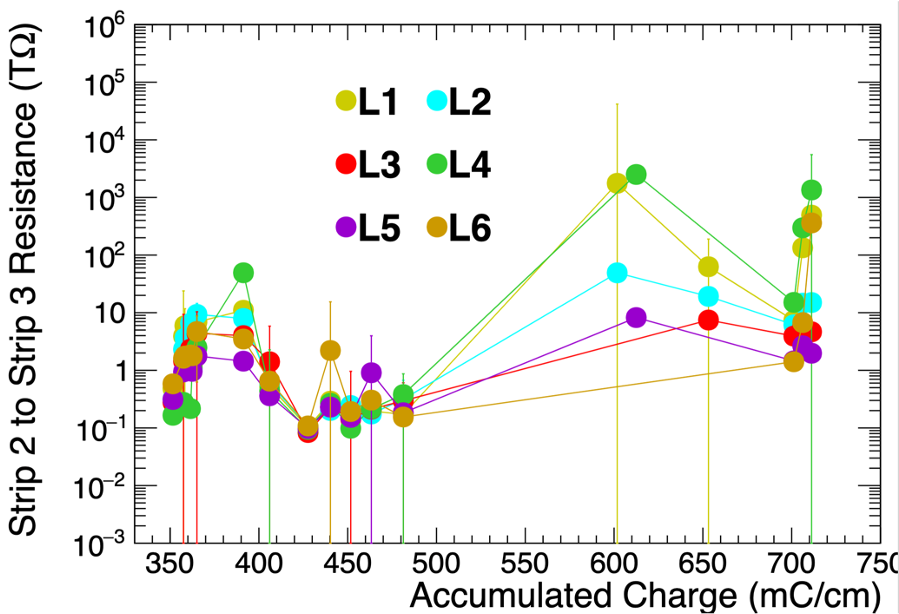
\includegraphics[width=0.8\textwidth]{figures/chapter05/s2s_ME11.png}
    \bicaption{\quad \centering ME1/1中$\CF$含量为2\%的Strip to Strip电阻测量结果}{\quad \centering The Strip to Strip resistance measurement results for ME1/1, which has  2\% $\CF$}
    \label{fig:c05f20}
\end{figure}

综上所述,将$\CF$的含量降低至2\%并没有使得探测器的Dark rate和电阻的测量发生明显的变化。但是,在对阳极丝进行显微镜扫描观测后,发现阳极丝表面出现了明显的氧化物沉积。因此,我们认为将$\CF$的含量降低至2\%可能存在一定风险,5\%的含量可能是比较好的选择。为此,对5\%$\CF$气体含量的测试正在进行中。